% =============================================================================
% CHAPITRE 1 - CINÉMATIQUE
% Partie 2 : La vitesse (toutes les définitions)
% Version maritime pour l'IMQ
% =============================================================================

% =============================================================================
\section{La vitesse}
% =============================================================================

\subsection{Importance de la vitesse}

La vitesse est l'une des grandeurs les plus fondamentales en physique. Elle quantifie \`a quel point un objet change de position rapidement. 

\begin{remarque}[title=La vitesse dans la vie quotidienne et professionnelle]
La vitesse est omnipr\'esente dans notre monde :
\begin{itemize}
    \item Un \textbf{conducteur} surveille son indicateur de vitesse pour respecter les limites
    \item Un \textbf{athl\`ete} cherche \`a optimiser sa vitesse de course ou de nage
    \item Un \textbf{pilote d'avion} doit maintenir une vitesse minimale pour ne pas d\'ecrocher
    \item Un \textbf{m\'edecin} mesure la vitesse de conduction nerveuse ou la vitesse du sang
    \item Un \textbf{officier de navigation} calcule les temps de travers\'ee, planifie les man\oe{}uvres et anticipe les situations de collision
\end{itemize}

Dans le contexte maritime, la vitesse est une donn\'ee critique : elle d\'etermine le temps d'arriv\'ee, la consommation de carburant, et la s\'ecurit\'e des man\oe{}uvres.
\end{remarque}

\subsection{Plusieurs d\'efinitions de la vitesse}

\begin{attention}[title=La vitesse n'est pas une seule chose!]
En physique, le mot \guillemotleft~vitesse~\guillemotright{} recouvre \textbf{plusieurs concepts distincts} :
\begin{itemize}
    \item La \textbf{vitesse scalaire moyenne} : quelle distance par unit\'e de temps?
    \item La \textbf{vitesse moyenne} : quel d\'eplacement par unit\'e de temps? (orient\'ee)
    \item La \textbf{vitesse instantan\'ee} : quelle vitesse \`a un instant pr\'ecis?
\end{itemize}

Ces trois d\'efinitions ne donnent \textbf{pas la m\^eme information}. Il est crucial de savoir laquelle utiliser selon le contexte.
\end{attention}

Commen\c{c}ons par la plus simple : la vitesse scalaire moyenne.

% =============================================================================
\subsection{Vitesse scalaire moyenne}
% =============================================================================

\begin{definition}[title=Vitesse scalaire moyenne]
La \textbf{vitesse scalaire moyenne} est le rapport entre la \textbf{distance totale parcourue} et l'intervalle de temps :
\begin{equationimportante}
\begin{equation}
v_{scalaire} = \frac{\text{distance parcourue}}{\Delta t} = \frac{d}{\Delta t}
\end{equation}
\end{equationimportante}

\begin{itemize}
    \item L'unit\'e SI est le \textbf{m\`etre par seconde} (\si{m/s})
    \item La vitesse scalaire moyenne est \textbf{toujours positive ou nulle}
    \item Elle repr\'esente l'\guillemotleft~effort r\'eel~\guillemotright{} de d\'eplacement
\end{itemize}
\end{definition}

\begin{remarque}[title=Unit\'es de vitesse courantes]
\begin{center}
\renewcommand{\arraystretch}{1.3}
\begin{tabular}{|l|l|}
\hline
\rowcolor{bleuclair}
\textbf{Unit\'e} & \textbf{\'Equivalence} \\
\hline
$\SI{1}{m/s}$ & Unit\'e SI de r\'ef\'erence \\
\hline
$\SI{1}{km/h}$ & $= \SI{0,278}{m/s} = \frac{1}{3,6}\,\si{m/s}$ \\
\hline
$\SI{1}{n\oe{}ud}$ (nd ou kn) & $= \SI{1,852}{km/h} = \SI{0,5144}{m/s}$ \\
\hline
\end{tabular}
\end{center}

Le \textbf{n\oe{}ud} est l'unit\'e de vitesse en navigation : $\SI{1}{n\oe{}ud} = \SI{1}{mille nautique/heure}$.
\end{remarque}

\begin{exemple}{Man\oe{}uvre d'un remorqueur}{}
Un remorqueur part du quai A, se rend au quai B ($\SI{800}{m}$), puis revient au quai C ($\SI{500}{m}$ de recul). La man\oe{}uvre totale prend $\SI{20}{minutes}$.

\textbf{Donn\'ees :}
\begin{itemize}
    \item Distance parcourue : $d = \SI{800}{m} + \SI{500}{m} = \SI{1300}{m}$
    \item Temps : $\Delta t = \SI{20}{min} \times \dfrac{\SI{60}{s}}{\SI{1}{min}} = \SI{1200}{s}$
\end{itemize}

\textbf{Vitesse scalaire moyenne :}
\[ v_{scalaire} = \frac{d}{\Delta t} = \frac{\SI{1300}{m}}{\SI{1200}{s}} = \SI{1,08}{m/s} \]

Conversion en n\oe{}uds :
\[ v_{scalaire} = \SI{1,08}{m/s} \times \frac{\SI{1}{n\oe{}ud}}{\SI{0,5144}{m/s}} = \SI{2,1}{n\oe{}uds} \]

Cette valeur repr\'esente bien l'activit\'e r\'eelle du remorqueur pendant ces 20 minutes.
\end{exemple}

% =============================================================================
\subsection{Vitesse moyenne}
% =============================================================================

La vitesse scalaire moyenne ne contient aucune information sur la \textbf{direction} du mouvement. Pour cela, on d\'efinit la vitesse moyenne.

\begin{definition}[title=Vitesse moyenne]
La \textbf{vitesse moyenne} $v_{moy}$ d'un objet est le rapport entre son \textbf{d\'eplacement} et l'intervalle de temps correspondant :
\begin{equationimportante}
\begin{equation}
v_{moy} = \frac{\Delta x}{\Delta t} = \frac{x_f - x_i}{t_f - t_i}
\end{equation}
\end{equationimportante}

\begin{itemize}
    \item C'est une grandeur \textbf{vectorielle} (en 1D : elle a un signe)
    \item Elle peut \^etre positive, n\'egative ou nulle
    \item Elle indique la \textbf{direction} du mouvement net
\end{itemize}
\end{definition}

\begin{remarque}[title=Signe de la vitesse moyenne]
Puisque $\Delta t$ est toujours positif, le \textbf{signe de la vitesse moyenne} est le m\^eme que celui du d\'eplacement :
\begin{itemize}
    \item $v_{moy} > 0$ : mouvement net dans le sens positif de l'axe
    \item $v_{moy} < 0$ : mouvement net dans le sens n\'egatif de l'axe
    \item $v_{moy} = 0$ : retour au point de d\'epart (d\'eplacement nul)
\end{itemize}
\end{remarque}

\begin{exemple}{Travers\'ee maritime}{}
Un cargo quitte le port de Rimouski \`a 8h00 et arrive \`a Sept-\^Iles \`a 20h00. La distance directe (d\'eplacement) entre les deux ports est de $\SI{180}{milles nautiques}$ vers l'est.

\textbf{Solution :}

Intervalle de temps : $\Delta t = 20h00 - 8h00 = \SI{12}{h}$

Vitesse moyenne :
\[ v_{moy} = \frac{\Delta x}{\Delta t} = \frac{\SI{+180}{NM}}{\SI{12}{h}} = \SI{+15}{n\oe{}uds} \]

Le signe positif indique que le mouvement est vers l'est (sens positif de l'axe).
\end{exemple}

\begin{pratiqueautonome}
Un cargo quitte le port de Matane à 6h00 et arrive à Baie-Comeau à 10h00. La distance directe entre les deux ports est de $\SI{52}{km}$ vers le nord-est.

Calculez la vitesse moyenne du cargo en km/h et en n\oe{}uds.

\espaceresolution[5cm]
\reponsepratique{$v_{moy} = \SI{13}{km/h} \approx \SI{7,0}{n\oe{}uds}$}
\end{pratiqueautonome}

\subsection{Pourquoi les deux sont importantes?}

\begin{center}
\renewcommand{\arraystretch}{1.4}
\begin{tabular}{|L{6cm}|L{6cm}|}
\hline
\rowcolor{bleuclair}
\textbf{Vitesse scalaire moyenne} $v_{scalaire}$ & \textbf{Vitesse moyenne} $v_{moy}$ \\
\hline
Bas\'ee sur la \textbf{distance parcourue} & Bas\'ee sur le \textbf{d\'eplacement} \\
\hline
Toujours positive ou nulle & Peut \^etre positive, n\'egative ou nulle \\
\hline
Repr\'esente l'\textbf{effort r\'eel} (\'energie d\'epens\'ee, carburant consomm\'e) & Repr\'esente le \textbf{r\'esultat net} (o\`u on s'est rendu) \\
\hline
N'indique pas la direction & \textbf{Indique la direction} du mouvement net \\
\hline
$v_{scalaire} = \dfrac{d}{\Delta t}$ & $v_{moy} = \dfrac{\Delta x}{\Delta t}$ \\
\hline
\end{tabular}
\end{center}

\begin{exemple}{Croisi\`ere Qu\'ebec -- \^Iles-de-la-Madeleine : comparaison}{}
Un navire de croisi\`ere quitte Qu\'ebec, fait escale aux \^Iles-de-la-Madeleine (\`a $\SI{650}{km}$), puis revient \`a Qu\'ebec. L'aller dure 2 jours et le retour dure 2 jours.

\begin{center}
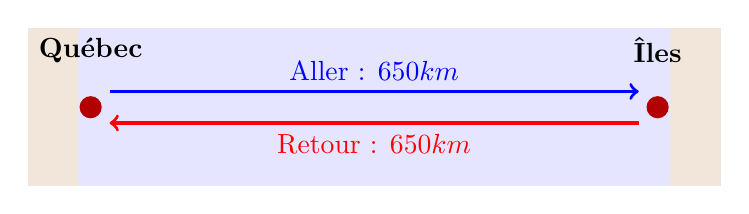
\begin{tikzpicture}[scale=0.8]
% Côte schématique
\fill[brown!20] (-0.5,-0.5) rectangle (0.3,2);
\fill[brown!20] (9.7,-0.5) rectangle (10.5,2);
% Mer
\fill[blue!10] (0.3,-0.5) rectangle (9.7,2);
% Villes
\fill[red!70!black] (0.5,0.75) circle (5pt);
\node[above] at (0.5,1.3) {\textbf{Qu\'ebec}};
\fill[red!70!black] (9.5,0.75) circle (5pt);
\node[above] at (9.5,1.3) {\textbf{\^Iles}};
% Trajets
\draw[very thick, blue, ->] (0.8,1) -- (9.2,1) node[midway, above] {Aller : $\SI{650}{km}$};
\draw[very thick, red, ->] (9.2,0.5) -- (0.8,0.5) node[midway, below] {Retour : $\SI{650}{km}$};
\end{tikzpicture}
\end{center}

\textbf{Vitesse scalaire moyenne :}
\[ v_{scalaire} = \frac{d}{\Delta t} = \frac{650 + 650}{4 \text{ jours}} = \SI{325}{km/jour} \approx \SI{13,5}{km/h} \]

\textbf{Vitesse moyenne :}
\[ v_{moy} = \frac{\Delta x}{\Delta t} = \frac{0}{4 \text{ jours}} = \SI{0}{km/h} \]

\begin{attention}
Les deux informations sont \textbf{compl\'ementaires} :
\begin{itemize}
    \item La vitesse scalaire ($\SI{13,5}{km/h}$) refl\`ete l'activit\'e r\'eelle du navire
    \item La vitesse moyenne (nulle) indique que le navire est revenu \`a son point de d\'epart
\end{itemize}
Aucune des deux n'est \guillemotleft~meilleure~\guillemotright{} --- elles r\'epondent \`a des questions diff\'erentes!
\end{attention}
\end{exemple}

\begin{exemple}{Navigation avec courant contraire}{}
Un traversier effectue l'aller-retour entre deux rives d'un fleuve s\'epar\'ees de $\SI{2}{km}$. \`A l'aller (avec le courant), il navigue \`a $\SI{12}{n\oe{}uds}$. Au retour (contre le courant), sa vitesse tombe \`a $\SI{8}{n\oe{}uds}$.

\textbf{Conversion des vitesses en km/h :}
\begin{align*}
v_{aller} &= \SI{12}{n\oe{}uds} \times \frac{\SI{1,852}{km/h}}{\SI{1}{n\oe{}ud}} = \SI{22,2}{km/h} \\[0.3cm]
v_{retour} &= \SI{8}{n\oe{}uds} \times \frac{\SI{1,852}{km/h}}{\SI{1}{n\oe{}ud}} = \SI{14,8}{km/h}
\end{align*}

\textbf{Calcul des temps :}
\begin{align*}
t_{aller} &= \frac{\SI{2}{km}}{\SI{22,2}{km/h}} = \SI{0,090}{h} = \SI{0,090}{h} \times \frac{\SI{60}{min}}{\SI{1}{h}} = \SI{5,4}{min} \\[0.3cm]
t_{retour} &= \frac{\SI{2}{km}}{\SI{14,8}{km/h}} = \SI{0,135}{h} = \SI{0,135}{h} \times \frac{\SI{60}{min}}{\SI{1}{h}} = \SI{8,1}{min}
\end{align*}

\textbf{Temps total :} $\Delta t = \SI{5,4}{min} + \SI{8,1}{min} = \SI{13,5}{min} = \SI{0,225}{h}$

\textbf{Vitesse scalaire moyenne :}
\[ v_{scalaire} = \frac{d}{\Delta t} = \frac{\SI{4}{km}}{\SI{0,225}{h}} = \SI{17,8}{km/h} = \SI{17,8}{km/h} \times \frac{\SI{1}{n\oe{}ud}}{\SI{1,852}{km/h}} = \SI{9,6}{n\oe{}uds} \]

\begin{attention}
La vitesse scalaire moyenne ($\SI{9,6}{n\oe{}uds}$) n'est \textbf{pas} la moyenne arithm\'etique des deux vitesses : $\dfrac{12 + 8}{2} = \SI{10}{n\oe{}uds}$.

C'est une erreur fr\'equente! La moyenne des vitesses ne donne la vitesse scalaire moyenne que si les \textbf{temps} de parcours sont \'egaux.
\end{attention}
\end{exemple}

\begin{pratiqueautonome}
Un remorqueur effectue un aller-retour entre deux quais séparés de $\SI{3}{km}$. À l'aller, il navigue à $\SI{10}{n\oe{}uds}$. Au retour, sa vitesse est de $\SI{6}{n\oe{}uds}$.

\begin{enumerate}[label=\alph*)]
    \item Calculez le temps total du trajet (en minutes).
    \item Calculez la vitesse scalaire moyenne. \textit{Attention au piège!}
\end{enumerate}

\espaceresolution[6cm]
\reponsepratique{a) $\Delta t \approx \SI{19,4}{min}$ \quad b) $v_{scalaire} \approx \SI{7,5}{n\oe{}uds}$ (et non $\SI{8}{n\oe{}uds}$!)}
\end{pratiqueautonome}

% =============================================================================
\subsection{Vitesse instantan\'ee}
% =============================================================================

Les vitesses moyenne et scalaire moyenne donnent une information \textbf{globale} sur un intervalle de temps. Mais que se passe-t-il \`a un \textbf{instant pr\'ecis}?

\begin{definition}[title=Vitesse instantan\'ee]
La \textbf{vitesse instantan\'ee} est la vitesse d'un objet \`a un instant pr\'ecis. C'est la vitesse moyenne calcul\'ee sur un intervalle de temps \textbf{infiniment petit} :
\begin{equationimportante}
\begin{equation}
v = \lim_{\Delta t \to 0} \frac{\Delta x}{\Delta t}
\end{equation}
\end{equationimportante}

En termes simples : c'est ce qu'affiche le \textbf{loch} (indicateur de vitesse) d'un navire ou le \textbf{compteur} d'une voiture \`a un instant donn\'e.
\end{definition}

\begin{remarque}[title=Vitesse moyenne vs vitesse instantan\'ee]
\begin{itemize}
    \item La \textbf{vitesse moyenne} caract\'erise le mouvement sur un \textbf{intervalle de temps}
    \item La \textbf{vitesse instantan\'ee} caract\'erise le mouvement \`a un \textbf{instant pr\'ecis}
    \item Si la vitesse est constante, alors $v_{instantan\'ee} = v_{moyenne}$ \`a tout instant
\end{itemize}
\end{remarque}

\begin{exemple}{Loch d'un navire}{}
Un navire acc\'el\`ere en quittant le port. Son loch affiche successivement :
\begin{itemize}
    \item \`A $t = \SI{0}{s}$ : $v = \SI{0}{n\oe{}ud}$
    \item \`A $t = \SI{60}{s}$ : $v = \SI{3}{n\oe{}uds}$
    \item \`A $t = \SI{120}{s}$ : $v = \SI{6}{n\oe{}uds}$
    \item \`A $t = \SI{180}{s}$ : $v = \SI{8}{n\oe{}uds}$
\end{itemize}

Chacune de ces valeurs est une \textbf{vitesse instantan\'ee}. La vitesse moyenne sur les 3 premi\`eres minutes n'est pas simplement $(0 + 3 + 6 + 8)/4$ --- il faudrait conna\^itre la position \`a chaque instant pour la calculer.
\end{exemple}

\begin{remarque}[title=Interpr\'etation graphique]
Sur un graphique position-temps $x(t)$, la vitesse instantan\'ee \`a un instant $t$ correspond \`a la \textbf{pente de la tangente} \`a la courbe en ce point.

Nous approfondirons cette interpr\'etation dans la section sur les graphiques.
\end{remarque}

% =============================================================================
\subsection{Vitesse surface et vitesse fond}
% =============================================================================

En navigation, on distingue deux vitesses importantes :

\begin{definition}[title=Vitesse surface et vitesse fond]
\begin{itemize}
    \item La \textbf{vitesse surface} est la vitesse du navire \textbf{par rapport \`a l'eau}. C'est ce qu'affiche le \textbf{loch}.
    \item La \textbf{vitesse fond} est la vitesse du navire \textbf{par rapport au sol}. C'est ce qu'affiche le \textbf{GPS}.
\end{itemize}

Ces deux vitesses diff\`erent lorsqu'il y a du \textbf{courant}. La relation est \textbf{vectorielle} :
\begin{equationimportante}
\begin{equation}
\vec{v}_{fond} = \vec{v}_{surface} + \vec{v}_{courant}
\end{equation}
\end{equationimportante}
\end{definition}

\begin{exemple}{Travers\'ee avec courant favorable}{}
Un navire affiche $\SI{12}{n\oe{}uds}$ au loch. Le courant de $\SI{2}{n\oe{}uds}$ pousse dans le m\^eme sens.

Vitesse fond : $v_{fond} = 12 + 2 = \SI{14}{n\oe{}uds}$

C'est cette vitesse qui d\'etermine l'heure d'arriv\'ee.
\end{exemple}
